\chapter{Scheduling della CPU}
\section{Scheduling}
\subsection{Fasi di eleborazion e di I/O}
Durante la vita di un processo, si alternano fasi di uso della \textbf{CPU} (CPU burst) e fasi di attesa per il completamento di operazioni di \textbf{I/O} (I/O burst). 

Possiamo distinguere due categorie di processi:

\begin{itemize}
    \item \textbf{Processi CPU-bound:} usano intensamente la CPU e interagiscono poco con i dispositivi di I/O (ad esempio un compilatore).
    \item \textbf{Processi I/O-bound:} usano poco la CPU ma fanno ampio uso dei dispositivi di I/O (ad esempio un editor o un browser).
\end{itemize}


\subsection{Lo Scheduler della CPU}
Consideriamo la situazione in cui un processo utente abbandona la \textbf{CPU}. Il Sistema Operativo (SO) si "sveglia" e deve decidere a quale, fra i processi in \textbf{Coda di Ready} (processi \emph{ready to run}), assegnare la CPU. Questa operazione è detta \textbf{Scheduling della CPU}, e viene gestita dal modulo del SO detto \textbf{scheduler}.

Quando interviene lo scheduler per scegliere il successivo processo a cui assegnare la CPU? Possiamo considerare quattro situazioni, che ci porteranno a definire i concetti di \textbf{scheduling con} e \textbf{senza diritto di prelazione}:

\begin{enumerate}

    \item Il processo che sta usando la CPU passa volontariamente dallo stato di running allo stato di waiting.
    \item Il processo che sa usando la CPU termina.
    \begin{itemize}
        \item In questi \textbf{due casi}, lo scheduler deve prendere un processo dalla coda di readt e mandarlo in eseucuzione
        \item \nt{Un sistema operativo che intervenga nei casi 1 e 2 è sufficiente per implementare il multi-tasking}
        \item \qs{}{Che succede se mandiamo in eseucuzione un programma che contiene una istruzione del tipo \texttt{while(true) printf("who's carr?")};}
        \item Il \textbf{SO} deve poter intervenire in modo da evitare che un processo si simpossessi della CPU, quindi...
    \end{itemize}
    \item Il processo che sta usando la CPU viene obbligato a passare dallo stato di running allo stato di ready
    \begin{itemize}
        \item Il passaggio non avviene mai \textbf{volontariamente}, il processo non vorrebbe lasciare la CPU a favore di qualcun'altro.
        \item Nei sistemi time sharing il SO non perde \textbf{mai} completamente il controllo del sistema
        \item Il SO mantiene il controllo della CPU attraverso un timer hardware, allo scadere del timer il controllo della CPU verrà restituito al SO, che sceglierà un processo dalla RQ un processo da mandare in esecuzione.
    \end{itemize}
    \item Un processo Px entra in coda di ready arrivando da una coda di wait oppure perchè è appena stato lanciato. 
    \qs{}{Perchè il SO interviene in questo caso?}
    \begin{itemize}
    \item \textbf{Primo:} i processi non si spostano autonomamente da una coda all’altra. È il Sistema Operativo (SO) che gestisce i loro \textbf{PCB} (Process Control Block). Ad esempio, quando il SO si accorge del completamento di un'operazione di I/O per cui il processo $P_x$ era in attesa, interviene per spostare (il PCB di) $P_x$ dalla \textbf{coda di wait} alla \textbf{coda di ready}.
    
    \item \textbf{Secondo:} se il processo $P_x$ risulta più "importante" rispetto al processo attualmente in esecuzione, il SO può decidere di togliere quest’ultimo dalla \textbf{CPU} e mandare in esecuzione $P_x$.
\end{itemize}
\end{enumerate}
Quando un sistema interviene solo nei casi 1 e 2 si parla di: \textbf{Scheduling senza (diritto di) prelazione}.\\
Quando un sistema interviene anche nei casi 3 e 4 si parla di: \textbf{Scheduling con (diritto di) prelazione}\\
Chiaramente, lo \textcolor{blue}{\textbf{scheduling preemptive}} è più sicuro per gli utenti, ma la sua implementazione richiede un \textcolor{purple}{sistema operativo} e un’\textcolor{purple}{architettura hardware} più sofisticati (ad esempio, un \textbf{timer dedicato}).\\
I moderni \textbf{sistemi operativi general purpose} usano tutti una qualche variante di \textcolor{blue}{\textbf{scheduling preemptive}}. Tuttavia, per applicazioni specifiche può essere sufficiente uno \textcolor{red}{\textbf{scheduling non-preemptive}}, permettendo l'uso di sistemi operativi più semplici e leggeri.\\
Lo \textcolor{blue}{\textbf{scheduling preemptive}} può portare a situazioni che necessitano di essere gestite con attenzione. Ad esempio, consideriamo un processo che deve compiere un’operazione di \textcolor{orange}{\textbf{I/O}} e chiama la relativa \textcolor{purple}{system call}. Il controllo viene trasferito al \textcolor{purple}{sistema operativo}, che inizia l’operazione per conto del processo utente. Nel frattempo, scade il timer e il controllo viene passato a un'altra porzione del codice del \textcolor{purple}{SO}.\\
Di conseguenza, una operazione delicata (altrimenti non sarebbe stata gestita dal \textcolor{purple}{SO}) viene interrotta a metà, e le \textcolor{orange}{\textbf{strutture dati}} potrebbero trovarsi in uno stato inconsistente poiché la system call di \textcolor{orange}{\textbf{I/O}} non ha finito di aggiornarle.\\
\qs{}{Cosa succede se ora la \textcolor{purple}{CPU} viene data a un altro processo utente che tenta di usare lo stesso dispositivo di \textcolor{orange}{\textbf{I/O}} che il processo precedente stava utilizzando? Quale semplice soluzione può essere adottata in tali casi?}
\nt{Vogliamo che il processo riesca a completare la richiesta al controller dell'I/O, niente di più}.
Mentre \textbf{Unix} è stato sviluppato fin dall’inizio come sistema di tipo {\textbf{preemptive}}, nei sistemi \textbf{Microsoft} la preemption è stata introdotta solo con \textbf{Windows 95}. Questo è dovuto al fatto che i sistemi operativi della famiglia \textbf{MS-Dos} sono nati come sistemi {\textbf{mono-utente}}, per i quali era sufficiente un sistema operativo più semplice. Inoltre, i primi sistemi per PC giravano su {CPU} semplici ed economiche, non dotate del supporto hardware necessario per implementare un sistema operativo {\textbf{preemptive}}.\\

\subsection{Il Dispatcher}
Quando lo scheduler ha scelto il processo a cui assegnare la CPU, interviene un altro modulo del SO, il \textit{dispatcher}, che:
\begin{itemize}
    \item Effettua l'operazione di \textit{context switch}.
    \item Effettua il passaggio del sistema in \textit{user mode}.
    \item Posiziona il \textit{PC} della CPU alla corretta locazione del programma da far ripartire.
\end{itemize}

Si definisce \textbf{Dispatch latency} il tempo impiegato per effettuare la commutazione da un processo ad un altro.

\section{Criteri di Scheduling}
Come abbiamo visto, lo scheduler della CPU interviene per assicurare il corretto funzionamento del sistema. Tuttavia, quando lo scheduler deve mandare in esecuzione un processo, quale criterio usa per scegliere tra tutti i processi presenti nella coda di ready? 

Si possono prendere in considerazione diversi obiettivi:

- Massimizzare l’\textbf{utilizzo} della CPU nell’unità di tempo, anche se questo dipende dal carico.
- Massimizzare il \textbf{throughput}, ossia la produttività del sistema, che si misura come il numero di processi completati in media in una certa unità di tempo.
- Minimizzare il \textbf{tempo di risposta}, cioè il tempo che intercorre da quando si avvia un processo a quando questo inizia effettivamente ad eseguire. Questo aspetto è particolarmente importante per i sistemi interattivi.

- Minimizzare il \textit{Turnaround time}: ossia il tempo medio di completamento di un processo, che va da quando entra per la prima volta nella \textit{ready queue} a quando termina.
- Minimizzare il \textit{Waiting time}: ossia la somma del tempo trascorso dal processo in \textit{ready queue}, ovvero quando il processo è pronto per eseguire il suo codice ma la CPU è occupata da un altro processo.

\qs{}{Che relazione c'è tra waiting time e turnaround time?}
\nt{Turnaround time - waiting time = tempo di esecuzione}

\section{Algoritmi di Scheudling}
\begin{itemize}
    \item \textbf{First Come, First Served (FCFS)}: Scheduling per ordine di arrivo.
    \item \textbf{Shortest Job First (SJF)}: Scheduling per brevità.
    \item \textbf{Priority Scheduling}: Scheduling per priorità.
    \item \textbf{Round Robin (RR)}: Scheduling circolare.
    \item \textbf{Multilevel Queue}: Scheduling a code multiple.
    \item \textbf{Multilevel Feedback Queue}: Scheduling a code multiple con retroazione.
\end{itemize}

\noindent \textbf{Nota Bene}: Nel seguito, considereremo processi con un unico \textit{burst} di CPU, senza \textit{burst} di I/O e con una durata espressa in generiche unità di tempo. Questo semplifica la comprensione degli algoritmi senza perdita di generalità.

\subsection{First Come First Served (FCFS)}
L'algoritmo \textit{First Come, First Served (FCFS)} è facile da implementare: gestisce la \textit{ready queue} (RQ) in modo FIFO (\textit{First In, First Out}). 
\begin{itemize}
    \item Il \textit{PCB} di un processo che entra nella \textit{RQ} viene inserito in fondo alla coda.
    \item Quando la CPU si libera, viene assegnata al processo il cui \textit{PCB} si trova in testa alla coda FIFO.
\end{itemize}

\noindent FCFS è un algoritmo non \textit{preemptive}, per cui non è adatto per i sistemi \textit{time-sharing}. Inoltre, con FCFS, il tempo di attesa per il completamento di un processo può risultare spesso molto lungo.

\subsubsection{Esempio}
Consideriamo tre processi che arrivano assieme al tempo t=0, e che entrano in CPU nell’ordine P1, P2, P3.
Come abbiamo già detto, i tre processi eseguono per un unico burst di CPU, e poi terminano.
\begin{table}[h]
    \centering
    \begin{tabular}{|c|c|}
        \hline
        \textbf{Process} & \textbf{Burst Time} \\
        \hline
        $P_1$ & 24 \\
        $P_2$ & 3 \\
        $P_3$ & 3 \\
        \hline
    \end{tabular}
    \caption{Process and Burst Time}
    \label{tab:process_burst_time}
\end{table}

Usiamo un diagramma di Gnatt per rappresentare questa situazione
\begin{figure}[h]
    \centering
    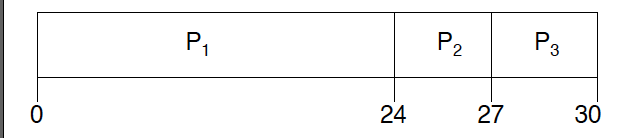
\includegraphics[width=0.5\linewidth]{images/FCFS_gnatt.png}
\end{figure}
Tempi di attesa $P_1 = 0; P_2 = 24; P_3 = 17$\\
Tempo medio di attesa $(0+24+27)/3 = 17$\\
Si dice che si è verificato \textbf{effetto convoglio}; i job più corti si sono dovuti accodare a quello lungo.
\bigskip
Se invece supponiamo che l'ordine di arrivo sia: P2, P3, P1
Tempi di attesa $P_1 = 6; P_2 = 0; P_3 = 3$\\
Tempo medio di attesa $(6+0+3)/3 = 3 \longleftrightarrow$ Molto meglio del caso precedente!\\

\subsubsection{Osservazioni}
Dunque, l'algoritmo \textit{FCFS} sembra comportarsi male nei confronti dei processi brevi. \\
Inoltre, \textit{FCFS} è pessimo per i sistemi \textit{time-sharing} poiché non garantisce un tempo di risposta ragionevole.\\
Ancora peggio, \textit{FCFS} non è adatto ai sistemi \textit{real-time} perché non è \textit{preemptive}.\\\\
Dall’esempio visto, sembra che le prestazioni migliorino facendo eseguire prima i processi più corti, indipendentemente dall’ordine di arrivo nella \textit{ready queue}. Tuttavia, questo apre la porta a nuovi problemi, che andremo a considerare.

\subsection{Shortest Job First (SJF)}
Si esamina la durata del prossimo \textit{burst} di CPU di ciascun processo in \textit{RQ} e si assegna la CPU al processo con il \textit{burst} di durata minima.\\
Il nome esatto di questo algoritmo è \textit{Shortest Next CPU Burst}.\\
 Può essere usato in modalità \textit{pre-emptive} e \textit{non pre-emptive}.\\
Nel caso \textit{preemptive}, se arriva in \textit{ready queue} un processo il cui \textit{burst time} è inferiore al tempo rimanente del processo attualmente in esecuzione, quest'ultimo viene interrotto e la CPU passa al nuovo processo. Questo schema è noto come \textit{Shortest-Remaining-Time-First} (SRTF).\\
\subsubsection{Esempio}
\begin{table}[ht]
    \centering
    \begin{tabular}{|c|c|c|}
        \hline
        \rowcolor[gray]{0.6} 
        Process & Arrival Time & Burst Time \\
        \hline
        $P_1$ & 0 & 7 \\
        $P_2$ & 2 & 4 \\
        $P_3$ & 4 & 1 \\
        $P_4$ & 5 & 4 \\
        \hline
    \end{tabular}
    \caption{Process, Arrival Time, and Burst Time}
    \label{tab:process_times}
\end{table}

\subsubsection{Non-preemptive}
Esempio:
\begin{figure}[ht]
    \centering
    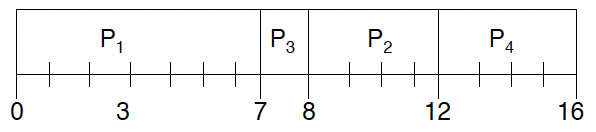
\includegraphics[width=0.2\linewidth]{images/SJF_nonpreemptive.png}
    \caption{Average waiting time $(0 + 6 + 3 + 7)/4 = 4$}
\end{figure}

\subsubsection{preemptive}
Esempio:
\begin{figure}[ht]
    \centering
    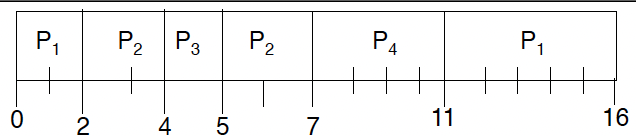
\includegraphics[width=0.2\linewidth]{images/SJF_preemptive.png}
    \caption{Average waiting time $(9 + 1 + 0 + 2/4 = 3$}
\end{figure}


\subsection{Osservazioni}
Si può dimostrare che l'algoritmo \textit{Shortest Job First} (SJF) è ottimale: spostando un processo breve prima di uno di lunga durata (anche se quest’ultimo è arrivato prima) si migliora l'attesa del processo breve più di quanto si peggiori quella del processo lungo. Di conseguenza, il tempo medio di attesa diminuisce, così come il \textit{turnaround time}.

SJF è ottimale: nessun altro algoritmo di \textit{scheduling} può produrre un tempo di attesa medio e un \textit{turnaround time} medio migliori. Tuttavia, c'è un problema...\\
Purtroppo, la durata del prossimo burst di CPU di un processo non è nota, il che rende l'algoritmo \textit{Shortest Job First} (SJF) non implementabile nella sua forma pura. SJF può al massimo essere approssimato utilizzando medie pesate per stimare la durata del prossimo burst di CPU di un processo, basandosi sulla durata dei burst di CPU precedenti.\nt{Da rivededere!!!!}\\

Lo \textit{scheduling} viene quindi eseguito sulla base di queste stime, fatte per tutti i processi nella \textit{Ready Queue} in un dato momento.\\
In sostanza, il \textit{First Come, First Served} (FCFS) è il peggiore degli algoritmi ragionevoli: funziona, ma spesso fornisce tempi medi di attesa e di \textit{turnaround} pessimi.\\

Al contrario, lo \textit{Shortest Job First} (SJF) è il migliore algoritmo possibile, ma non è implementabile nella pratica, e possiamo solo usarlo per fare simulazioni con processi i cui burst di CPU siano noti a priori.\\

FCFS e SJF rappresentano i due estremi di uno spettro di possibili algoritmi di \textit{scheduling}. Un algoritmo di \textit{scheduling} sarà tanto migliore quanto più le sue prestazioni si allontanano da quelle di FCFS e si avvicinano a quelle di SJF.

\subsection{Scheduling a Priorità}
SJF è un tipo scheduling a priorità, la durata del prossimo burst time è la priorità corrente di ogni processo.
FCFS è uno scheduling a priorità, viene data più alta ai primi che arrivano
In generale, il calcolo della priorità dei processi può essere:
\begin{itemize}
    \item \textbf{Interna al sistema}: calcolata dal SO sulla base del comportamento di ogni processo (ad esempio, in base alle risorse usate fino a quel momento da un processo).
    \item \textbf{Esterna al sistema}: assegnata con criteri esterni al SO (ad esempio, una priorità che cambia in base a quale utente ha lanciato il processo).
\end{itemize}

Lo \textit{scheduling} a priorità può essere implementato sia in modalità \textbf{preemptive} che \textbf{non preemptive}.

\subsubsection{Starvation e aging}
\qs{Problema}{Che succede se un processo in RQ ha sempre una priorità peggiore di qualche altro processo in RQ?}
Il processo potrebbe non essere mai scelto dallo scheduler. Questo fenomeno è noto come \textbf{starvation} (muore di fame...). 

Per risolvere il problema della \textit{starvation}, si usa un meccanismo chiamato \textbf{aging}: il SO aumenta progressivamente la priorità di un processo $P_x$ man mano che $P_x$ passa tempo nella Ready Queue (RQ). In questo modo, prima o poi, $P_x$ avrà una priorità maggiore rispetto agli altri processi e verrà scelto dallo scheduler.

\qs{}{Gli algoritmi \textit{FCFS}, \textit{SJF preemptive} e \textit{non preemptive} possono provocare starvation?}
\nt{Per SJF, arrivano sempre processi con burst piccolissimi e quindi un processo più grande aspetterà (Sia per preemptive che non)}

\subsection{Scheduling Round Robin (RR)}
Ogni processo ha a disposizione una certa quantità di tempo di CPU, chiamata \textbf{quanto di tempo} (valori ragionevoli vanno da 10 a 100 millisecondi). Per ora, assumiamo un unico quanto di tempo prefissato assegnato a tutti i processi. 

Se entro questo arco di tempo il processo non lascia volontariamente la CPU, viene interrotto e rimesso nella Ready Queue (RQ). La RQ è vista come una coda circolare, e si verifica una sorta di \textit{“girotondo”} di processi.

L'implementazione dello scheduling \textbf{round robin} è concettualmente molto semplice:
\begin{itemize}
    \item Lo scheduler sceglie il primo processo in RQ (ad esempio secondo un criterio FCFS).
    \item Lancia un timer inizializzato al quanto di tempo.
    \item Passa la CPU al processo scelto.
\end{itemize}

Se il processo ha un CPU burst minore del quanto di tempo, il processo rilascierà la CPU volontariamente prima dello scadere del tempo assegnatogli. Se invece il CPU burst del processo è maggiore del quanto di tempo, allora:
\begin{itemize}
    \item Il timer scade e invia un interrupt.
    \item Il SO riprende il controllo della CPU.
    \item Togliere la CPU al processo in esecuzione e metterlo in fondo alla RQ.
    \item Prendere il primo processo in RQ e ripetere tutto.
\end{itemize}

\subsubsection{Osservazioni}
Se ci sono \( n \) processi in coda ready e il quanto di tempo è \( q \), allora ogni processo riceve \( \frac{1}{n} \) del tempo della CPU e nessun processo aspetta per più di \( (n-1)q \) unità di tempo.

Il \textbf{Round Robin} è l'algoritmo di scheduling naturale per implementare il time sharing ed è quindi particolarmente adatto per i sistemi interattivi: nel caso peggiore, un utente non aspetta mai più di \( (n-1)q \) unità di tempo prima che il suo processo venga servito.

Come vedremo negli esempi di casi reali, il SO adotta poi ulteriori misure per migliorare il tempo di risposta dei processi interattivi.

\subsection{Esempio}
\begin{table}[h]
    \centering
    \begin{tabular}{|c|c|}
        \hline
        \textbf{Process} & \textbf{Burst Time} \\
        \hline
        $P_1$ & 53 \\
        $P_2$ & 17 \\
        $P_3$ & 68 \\
        $P_4$ & 24 \\
        \hline
    \end{tabular}
    \caption{Process and Burst Time}
    \label{tab:process_burst_time}
\end{table}
\begin{figure}[h]
    \centering
    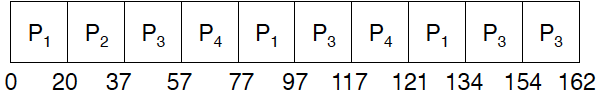
\includegraphics[width=0.25\linewidth]{images/RR_20.png}
\end{figure}
Tipicamente sia ha un \textit{turnaround} medio maggiore di SJF, ma un migliore \textbf{tempo di risposta}
Le prestazioni del \textbf{Round Robin} dipendono molto dal valore del quanto di tempo \( q \) scelto:
\begin{itemize}
    \item \( q \) tendente a infinito rende \textbf{RR} uguale a \textbf{FCFS}.
    \item \( q \) tendente a zero produce un maggior effetto di “parallelismo virtuale” tra i processi.
    \item Tuttavia, questo aumenta il numero di context switch e, di conseguenza, l'overhead.
\end{itemize}

\subsection{Scheduling a Code Multiple}

I processi possono essere suddivisi in classi differenti:
\begin{itemize}
    \item \textbf{foreground}: processi interattivi (es. un editor)
    \item \textbf{background}: processi che non interagiscono con l'utente
    \item \textbf{batch}: processi la cui esecuzione può essere differita
\end{itemize}

La risorsa di esecuzione (RQ) può essere partizionata in più code:
\begin{itemize}
    \item I processi vengono inseriti in una coda basata sulle loro proprietà
    \item Ogni coda viene gestita con lo scheduling appropriato
\end{itemize}
Ogni coda ha quindi la sua politica di scheduling, ad esempio:
\begin{itemize}
    \item \textit{foreground}: \textbf{RR}
    \item  \textit{background e batch}: \textit{FCFS}
\end{itemize}
\qs{}{Ma come si sceglie fra le code?
\begin{itemize}
    \item \textbf{Scheduling a priorità fissa}: servire prima tutti i processi nella coda foreground e poi quelli in background e batch. Possibilità di \textbf{starvation}.
    \item  \textbf{Time slice}: ogni coda ha una certa quantità di tempo di CPU, ad esempio: 80\% alla coda foreground e 20\% alla coda background e batch
\end{itemize}
}

\begin{figure}[h]
    \centering
    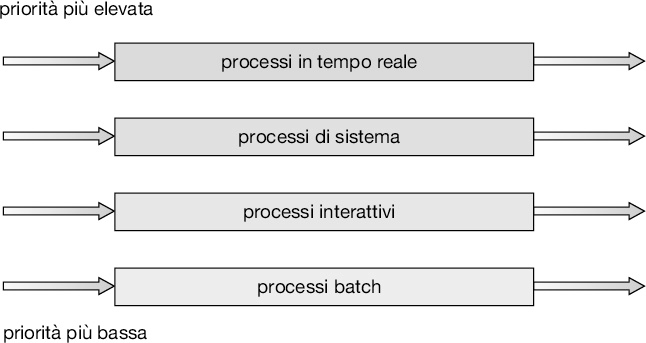
\includegraphics[width=0.5\linewidth]{images/Scheduling_multiple_queue.png}
    \caption{Partizionamento dei processi in più code}
\end{figure}

\subsection{Scheduling a Code Multilivello con retroazione (MFQS)}
Il tipo più generale di algoritmo di scheduling è lo \textbf{scheduling a code multilivello con retroazione} (MFQS), utilizzato dai sistemi operativi moderni.

\begin{itemize}
    \item L'assegnamento di un processo a una coda non è fisso: i processi possono essere spostati dal SO per adattarsi alla lunghezza del loro \textit{CPU burst}.
    \item Ogni coda è gestita con lo scheduling più adatto ai processi in essa contenuti.
\end{itemize}

Esempio (fig. 5.4):
\begin{figure}[h]
    \centering
    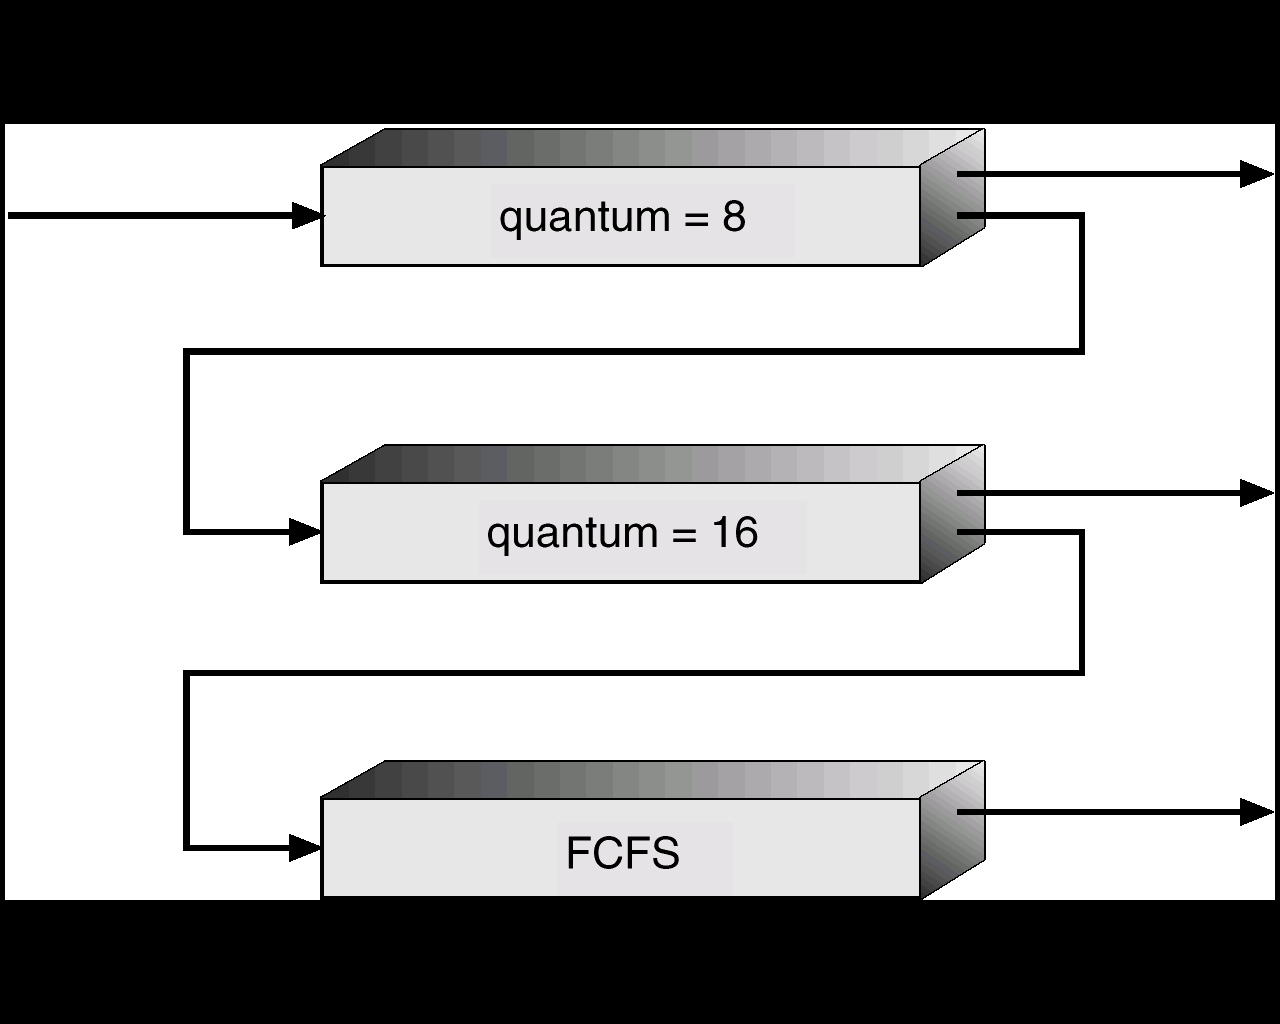
\includegraphics[width=0.25\linewidth]{images/MFQS.png}
    \caption{Esempio di MFQS}
    \label{fig:5.4}
\end{figure}
\begin{itemize}
    \item Le prime due code sono gestite con \textit{Round Robin (RR)}, mentre la terza con \textit{First-Come, First-Served (FCFS)}.
    \item Quando un processo nasce, è inserito nella prima coda ($q=8$). Se non finisce il \textit{CPU burst} entro il quanto, viene retrocesso alla coda successiva.
    \item È definita una priorità tra le code, che sono gestite con \textit{preemption}.
\end{itemize}

La politica MFQS è caratterizzata da:
\begin{itemize}
    \item numero di code
    \item algoritmo di scheduling per ogni coda
    \item quando declassare o promuovere un processo
    \item in che coda inserire un processo quando arriva (dall'esterno o da un \textit{I/O burst})
\end{itemize}

MFQS è il tipo di scheduling più generale e complesso da configurare.


\section{Scheduling per sistemi multi-core}
Sono ormai comuni le architetture con CPU a 2, 4, 8 core, Sono, in sostanza, dei piccoli sistemi multiprocessore in cui sullo stesso chip sono presenti due o più core che vedono la stessa memoria principale e condividono un livello di cache.
La presenza di più “unità di esecuzione” dei processi, permette naturalmente di aumentare le prestazioni della macchina, posto che il SO sia in grado di sfruttare a pieno ciascun core.

I sistemi operativi moderni prevedono la \textbf{multielaborazione simmetrica} (SMP), in cui uno scheduler gira su ciascun core.
\begin{itemize}
    \item I processi "ready to run" possono essere inseriti in una coda comune oppure in una coda separata per ogni core.
    \item Lo scheduler di ciascun core sceglie un processo dalla propria coda e lo manda in esecuzione.
\end{itemize}

Un aspetto chiave nei sistemi multi-core è il \textbf{bilanciamento del carico}, ossia la distribuzione omogenea dei processi tra i core.
\begin{itemize}
    \item Con una coda comune, il bilanciamento è automatico: un core inattivo prende un processo dalla coda comune.
    \item Con code separate per ogni core, è necessario un meccanismo per spostare i processi dai core sovraccarichi a quelli scarichi. \textbf{Questo è il processo preferito dai moderni SO}
    \item Ad esempio, Linux SMP attiva il bilanciamento del carico ogni 200 ms o quando una coda si svuota.
\end{itemize}

Spostare un processo tra core può causare rallentamenti dovuti alla \textbf{cache}, poiché il processo potrebbe non trovare i dati nelle cache private del nuovo core.
Non trovandoli è costretto a spendere più tempo per recuperarli, se va bene, dalla cache L3, che condivide con gli altri core. Per evitare questo problema, specifiche \textit{system call} permettono di vincolare un processo a un certo core.

\subsection{Esempio}

\begin{figure}[h]
    \centering
    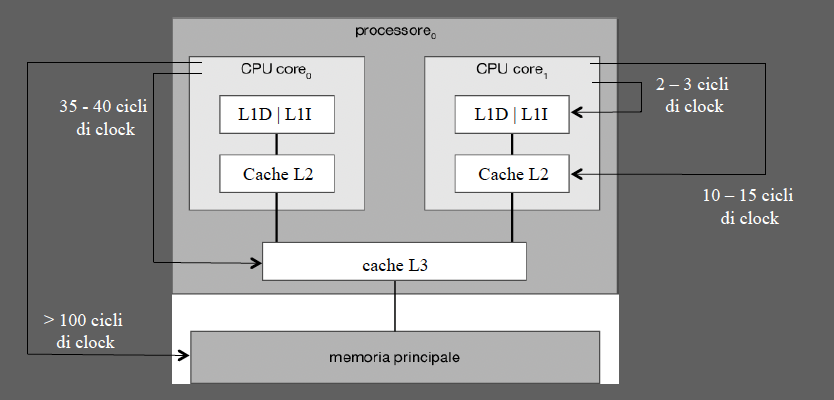
\includegraphics[width=0.5\linewidth]{images/Scheduling_multi_core_i7.png}
    \caption{Scheduling example}
    \label{fig:schedi7}
\end{figure}
Qui vediamo il costo in cicli di clock necessari per accedere ad un dato/istruzione in un certo livello di cache. I valori si riferiscono ad un processore Intel core i7, ma valgono per la maggior parte dei processori moderni \ref{fig:schedi7}.

\section{Esempi di sistemi operativi}
Solaris utilizza uno \textbf{scheduling a priorità con code multiple a retroazione}, suddividendo i processi in 4 classi:
\begin{enumerate}
    \item real time (priorità maggiore)
    \item sistema
    \item interattiva
    \item time sharing (priorità minore)
\end{enumerate}

\begin{itemize}
    \item Un processo usa la CPU fino a quando non termina, va in \textit{wait}, esaurisce il quanto di tempo o è preemptato.
    \item I processi delle classi \textit{time sharing} e \textit{interattiva} hanno criteri di scheduling simili con 60 livelli di priorità.
    \item La priorità di un processo e il quanto di tempo assegnato sono inversamente proporzionali. Se un processo esaurisce il quanto, la sua priorità viene abbassata; al contrario, se si sospende prima, la priorità aumenta.
\end{itemize}

Il comportamento del processo stabilisce se rientra nella classe \textit{time sharing} (priorità 0-49) o \textit{interattiva} (priorità 50-59)
% Requires: \usepackage{colortbl}
\begin{table}[h]
    \centering
    \begin{tabular}{|c|c|c|c|}
    \hline
    \rowcolor{gray} \textbf{Priorità corrente} & \textbf{Quanto di tempo} & \textbf{Nuova priorità} & \textbf{Nuova priorità} \\
    \rowcolor{gray} & \textbf{(millisecondi)} & \textbf{(quanto esaurito)} & \textbf{(quanto non esaurito)} \\
    \hline
    0 & 200 & 0 & 50 \\
    \hline
    20 & 120 & 10 & 52 \\
    \hline
    30 & 80 & 25 & 53 \\
    \hline
    59 & 20 & 49 & 59 \\
    \hline
    \end{tabular}
    \caption{Tabella delle priorità e tempi}
    \label{tab:pri_tempi}
\end{table}

La \textbf{priorità corrente} di un processo determina il \textbf{quanto di tempo} che gli viene assegnato. Priorità e tempo assegnato sono inversamente proporzionali.

\begin{itemize}
    \item \textbf{Quanto esaurito}: se un processo ha esaurito tutto il quanto di tempo senza sospendersi, la sua nuova priorità sarà più bassa, e in futuro riceverà un quanto di tempo più lungo.
    \item \textbf{Quanto non esaurito}: se un processo si sospende prima di consumare tutto il quanto, la sua nuova priorità sarà più alta, e in futuro riceverà un quanto di tempo più breve.
\end{itemize}


\begin{itemize}
    \item I processi \textit{real time} e di \textit{sistema} hanno priorità fissa, superiore a quella delle classi \textit{time sharing} e \textit{interattiva}.
    \item Lo scheduler assegna la CPU al processo con la priorità globale più alta e, in caso di parità, utilizza il \textit{Round Robin} (RR).
    \item L'algoritmo è \textbf{preemptive}: un processo attivo può essere interrotto da uno con priorità globale più alta.
\end{itemize}

\subsection{Lo scheduling in Windows}
Lo scheduling in Windows è basato su \textbf{priorità con retroazione e prelazione}, utilizzando 32 livelli di priorità:
\begin{itemize}
    \item I processi \textit{real-time} hanno priorità da 16 a 31.
    \item I processi non real-time hanno priorità da 1 a 15, con 0 riservato.
\end{itemize}

Per i processi non real-time:
\begin{itemize}
    \item Quando un processo nasce, ha una priorità iniziale di 1.
    \item Lo scheduler assegna la CPU al processo con la priorità più alta, usando \textit{Round Robin} (RR) in caso di parità.
    \item Se un processo va in \textit{wait} prima di esaurire il quanto di tempo, la sua priorità viene aumentata (fino a 15), a seconda dell'evento in attesa (maggiore incremento per input da tastiera, minore per I/O da disco).
    \item Se un processo esaurisce il quanto di tempo, la sua priorità viene abbassata, ma mai sotto 1.
\end{itemize}

Questa strategia favorisce i processi interattivi (mouse e tastiera) per migliorare il \textbf{tempo di risposta}. Inoltre, quando un processo passa in \textit{foreground}, il suo quanto di tempo viene moltiplicato per 3, consentendogli di mantenere la CPU per un periodo più lungo.

\subsection{Lo Scheduling in Linux}
Dal 2007, Linux utilizza il \textbf{Completely Fair Scheduler} (CFS) come algoritmo di scheduling predefinito.

Il CFS distribuisce equamente il tempo di CPU tra i processi \textit{ready to run}, seguendo l'assunzione che se ci sono $N$ processi attivi, ciascun processo dovrebbe ricevere esattamente $\frac{1}{N}$ del tempo di CPU.

Ad ogni \textit{context switch}, il CFS ricalcola per quanto tempo assegnare la CPU a un processo $P$, in modo che tutti abbiano la stessa quantità di tempo CPU. Siano:
\begin{itemize}
    \item $P.\texttt{expected\_run\_time}$: il tempo di CPU spettante a $P$;
    \item $P.\texttt{vruntime}$: il tempo di CPU già consumato da $P$;
    \item $P.\texttt{due\_cputime}$: il tempo di CPU che ancora spetta a $P$.
\end{itemize}

Dunque:
\[
P.\texttt{vruntime} = P.\texttt{expected\_run\_time} - P.\texttt{due\_cputime}
\]
La CPU viene assegnata al processo con il valore più basso di $P.\texttt{vruntime}$, ossia al processo che ha usato meno CPU fino a quel momento.

Nel CFS, i processi \textit{ready to run} non sono organizzati in code di scheduling, ma come nodi in un \textbf{red-black tree (R-B tree)}, che consente operazioni di ricerca, inserimento e cancellazione con complessità computazionale $O(\log n)$, dove $n$ è il numero di nodi.

Negli alberi R-B il nodo più a sinistra è sempre quello col valore chiave più basso, e nel CFS i processi sono inseriti nel R-B tree usando come chiave P.vruntime.
Dunque, il processo associato al nodo più a sinistra ha il valore P.vruntime più basso, cioè è il processo che ha usato la CPU per meno tempo, e al context switch sarà scelto per entrare in esecuzione.

\begin{figure}
    \centering
    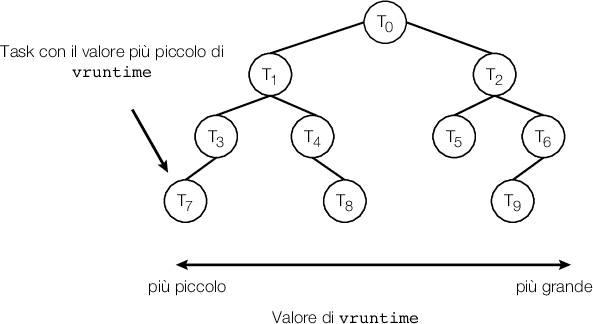
\includegraphics[width=0.5\linewidth]{images/Scheduling-Linux-Tree.png}
    \caption{vrun time tree}
    \label{fig:v-runtimetree}
\end{figure}
